\subsection{Sele\c{c}\~ao e entrega de conte\'udo}
\paragraph{} Dentro de uma CDN temos que  nos preocupar com a forma como esse conte\'udo vai catalogado, armazenado e distribu\'ido dentro da rede, o que vimos no item \ref{section:protocolos_interacoes}, como tamb\'em temos que nos preocupar como esse conte\'udo vai chegar at\'e o cliente (usu\'ario) da forma mais otimizada poss\'ivel, ou seja, o servidor o qual vai fornecer as informa\c{c}\~oes para ele ser\'a o mais perto ou mais r\'apido. 
\paragraph{} Temos que destacar tamb\'em a import\^ancia da otimiza\c{c}\~ao do fluxo de informa\c{c}\~ao pela rede. Visto que quanto maior o tr\'afico de informa\c{c}\~ao pela rede significa que a informa\c{c}\~ao est\'a mais distante do usu\'ario e tamb\'em que vai ter um custo maior pela troca intensa de informa\c{c}\~ao. 
\paragraph{} Segundo \cite{krishnamurthy2001use}, na tentativa de otimizar o redirecionamentos de URL para o usu\'ario se sacramentou dois tipos de t\'ecnicas de redirecionamentos:
\begin{itemize}
	\item Full - site
	\item Partial - site
\end{itemize}

\subsubsection{Full - site}
\paragraph{} Na t\'ecnica de Full-site todo o conte\'udo \'e entregado ao usu\'ario de um servidor ponta \'unico. Ou seja, o usu\'ario faz uma requisi\c{c}\~ao ao servidor principal, onde o mesmo processa um algoritmo de roteamento para encontrar o servidor ponta que melhor se enquadra como resposta, e ent\~ao retorna ao usu\'ario o endere\c{c}o onde ent\~ao ser\'a consumido por fim todas as informa\c{c}\~oes requisitadas. 
\paragraph{} \'E importante salientar que essa t\'ecnica \'e amplamente utilizada por servi\c{c}os que fazem pouco uso de dados da rede. Uma p\'agina est\'atica da web, por exemplo, se encaixaria perfeitamente nesse contexto. Visto que possui baixo grau de modifica\c{c}\~oes e seu tamanho \'e pequeno perto de outros tipos de m\'idias que circulam na web.

\subsubsection{Partial - site}
\paragraph{} J\'a redirecionamentos do tipo Partial-sites os servideores principais retornam para o usu\'ario uma parte do conte\'udo e disparam, automaticamente, um algoritmo de roteamento para encontrar o restante da informa\c{c}\~ao e retornar ao usu\'ario. Conforme podemos ver na figura \ref{figura:entrega_conteudo}
\begin{figure}[H]
\caption{Entrega de conte\'udo}
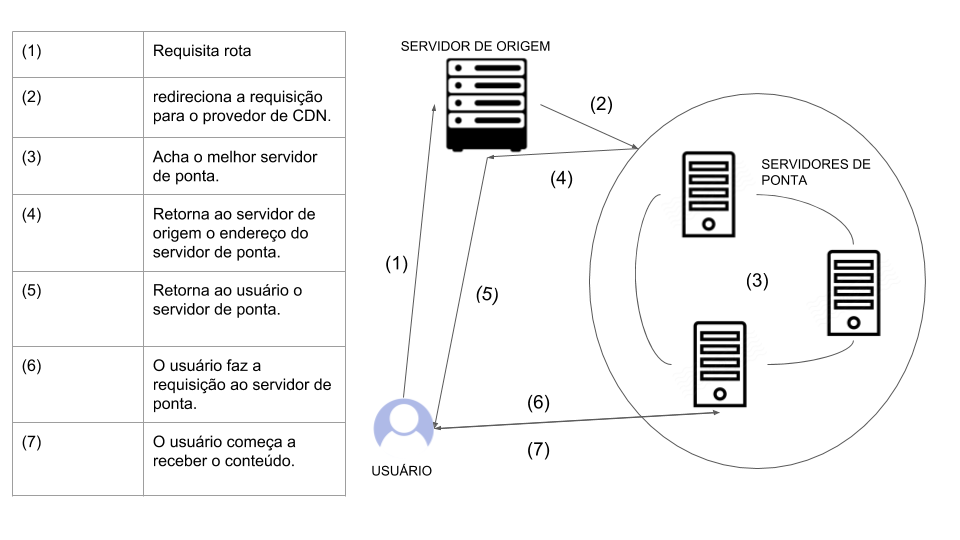
\includegraphics[height=9cm]{Figuras/entrega_conteudo.png} 
\label{figura:entrega_conteudo}
\end{figure}
\paragraph{}  Nela podemos ver que todo o processo acontece em, basicamente, 5 etapas. (1) o usu\'ario faz uma requisi\c{c}\~ao ao servidor principal, depois, em (2) o servidor principal retornar um html com as principais informa\c{c}\~oes e dispara automaticamente (3) um processo de roteamento (4) para buscar o melhor servidor e retornar (5) para o usu\'ario os conte\'udos.
\paragraph{} Entretanto h\'a em (4) diversas formas de fazer esse roteamento quanto a distribui\c{c}\~ao do conte\'udo pela rede e quanto a aglomera\c{c}\~ao desse conte\'udo dentro do servidores de cache. 
\paragraph{} Tipo de distribui\c{c}\~ao nada mais \'e do que a forma como o conte\'udo vai ser disperso na rede, como esse conte\'udo vai se aproximar do n\'o que est\'a mais perto do usu\'ario. 

Os tipos de distribui\c{c}\~ao mais frequentemente utilizados s\~ao:
\begin{itemize}
	\item Emp\'irico
	\item Popularidade
\end{itemize}

\paragraph{} Emp\'irico trata, como o pr\'oprio nome diz, de uma forma de distribui\c{c}\~ao sem nenhum conhecimento espec\'ifico a respeito, utilizando-se apenas um conhecimento experimental de onde seria melhor posicionado o conte\'udo.
\paragraph{} Em um esquema baseado em popularidade a distribui\c{c}\~ao \'e feita conforme a notoriedade. Ou seja, quanto mais a requisi\c{c}\~ao do conte\'udo mais ele vai ficar nos servidores de ponta perto do usu\'ario.
\paragraph{} Ambos esquemas n\~ao s\~ao necessariamente excludentes, pode-se inicialmente aplicar a forma empir\'ica para gerar dados a respeito da distribui\c{c}\~ao e depois utilizar esses dados para aplicar o modo de popularidade.
	
\paragraph{} Tamb\'em existe as formas de aglomera\c{c}\~oes de conte\'udo. Isso existe porque os conte\'udos podem ser conjuntos de objetos ou objetos independentes. 
As formas de aglomera\c{c}\~oes s\~ao:
\begin{itemize}
	\item Objeto
	\item Conjunto de objetos
\end{itemize}

\paragraph{} Aglomera\c{c}\~ao por objeto vai juntar os objetos mais selecionados e distribui-los individualmente entre os servidores. J\'a por conjunto de objetos ele vai separa-los em grupos e distribui-los em conjuntos. 
\paragraph{} Podemos exemplicar da seguinte forma: Em um site temos v\'arios elementos, temos o HTML, temos o CSS e temos a media de um v\'ideo qualquer. Podemos separar da seguinte forma temos 3 elementos onde 2 deles s\~ao altamente dependentes(HTML e CSS) e temos u que pode ser diferente em cada regi\~ao do pa\'is que \'e o v\'ideo. Ent\~ao podemos misturar as formas de aglomera\c{c}\~oes, para o HTML e para o CSS agrupamos em conjuntos de objetos, e para o v\'ideo fazemos a aglomera\c{c}\~ao por objeto, j\'a que ser\'a distribu\'ido de maneira independente nos servidores.

\paragraph{} Analisando os tipos se perceber que nenhuma das op\c{c}\~oes s\~ao excludentes entre s\'i. Pode-se combinar quaisquer tipo de distribui\c{c}\~ao e aglomera\c{c}\~ao e tamb\'em. As escolhas v\~ao depender das necessidades de cada aplica\c{c}\~ao.\'E necess\'ario uma an\'alise minuciosa de cada aplica\c{c}\~ao para chegar em um veredito da melhor abordagem.
\subsubsection{VOD}
\paragraph{VOD - Video on Demand} - Segundo \cite{garfinkle1996video}, \'e um sistema de que proporciona uma interface de comunica\c{c}\~ao com o usu\'ario de produtos dispon\'iveis de uma esta\c{c}\~ao central remota.
\newline \'E um sistema muito utilizado por operadoras de conte\'udo onde \'e o cliente que decide o hor\'ario que ir\'a consumir determinado conte\'udo.
\newline Isso permite que pessoas que antes tinham que esperar hor\'ario certo para consumir determinado conte\'udo, agora podem a qualquer momento e em qualquer lugar fazer uso do mesmo. Visto que est\'a dispon\'ivel online.
\paragraph{Microsoft Smooth Streaming} \'E um sistema de consumo de v\'ideo onde a qualidade do v\'ideo transmitida vai ser definida conforme a qualidade da banda dispon\'ivel. Clientes que possuem alta disponibilidade de banda ter\~ao maior qualidade do v\'ideo. 
\newline Para conseguir tocar um v\'ideo nesse formato o player do usu\'ario tem que ser capaz de interpretar um manifesto que cont\'em dentro de outras coisas, o caminho de onde est\'a localizado a m\'idia desejada. 
\newline J\'a para consegui fazer a transi\c{c}\~ao de qualidade o v\'ideo \'e quebrado em pequenos peda\c{c}os chamados de "chuncks". Ent\~ao, conforme \'e verificada um aumento ou decremento da banda dispon\'ivel \'e s\'o o player come\c{c}ar q consumir chuncks de qualidade diferente da atual e assim o usu\'ario j\'a passar\'a v\^e a diferen\c{c}a significante na tela. 
\newline No artigo \cite{zambelli2009iis} podemos v\^e todas as aplica\c{c}\~oes e implica\c{c}\~oes dessa forma de consumo de m\'idia.
\subsubsection{Exemplo}
\paragraph{} Agora vamos ilustrar com um exemplo mais pr\'atico. Utilizaremos uma requisi\c{c}\~ao de uma URL de um VOD(Video On Demand) onde a parte de roteamento \'e feita no usu\'ario. A aplica\c{c}\~ao do usu\'ario faz uma requisi\c{c}\~ao \`a CDN e enquanto o cabe\c{c}alho da resposta n\~ao for 200 ele vai ler um campo dentro do cabe\c{c}alho de resposta e fazer uma nova requisi\c{c}\~ao. A figura (FAZER A FIGURA) ilustra a situa\c{c}\~ao.

Como podemos observar na figura \ref{figura:exemplo_vod_1} a aplica\c{c}\~ao manda para o player a url associada ao VOD que \'e respons\'avel por responder com o caminho oficial, ou intermedi\'ario, do manifesto. Na figura \ref{figura:exemplo_vod_1} ele est\'a localizado no campo "play\_info" da requisi\c{c}\~ao.
\begin{figure}[H]
\caption{exemplo VOD}
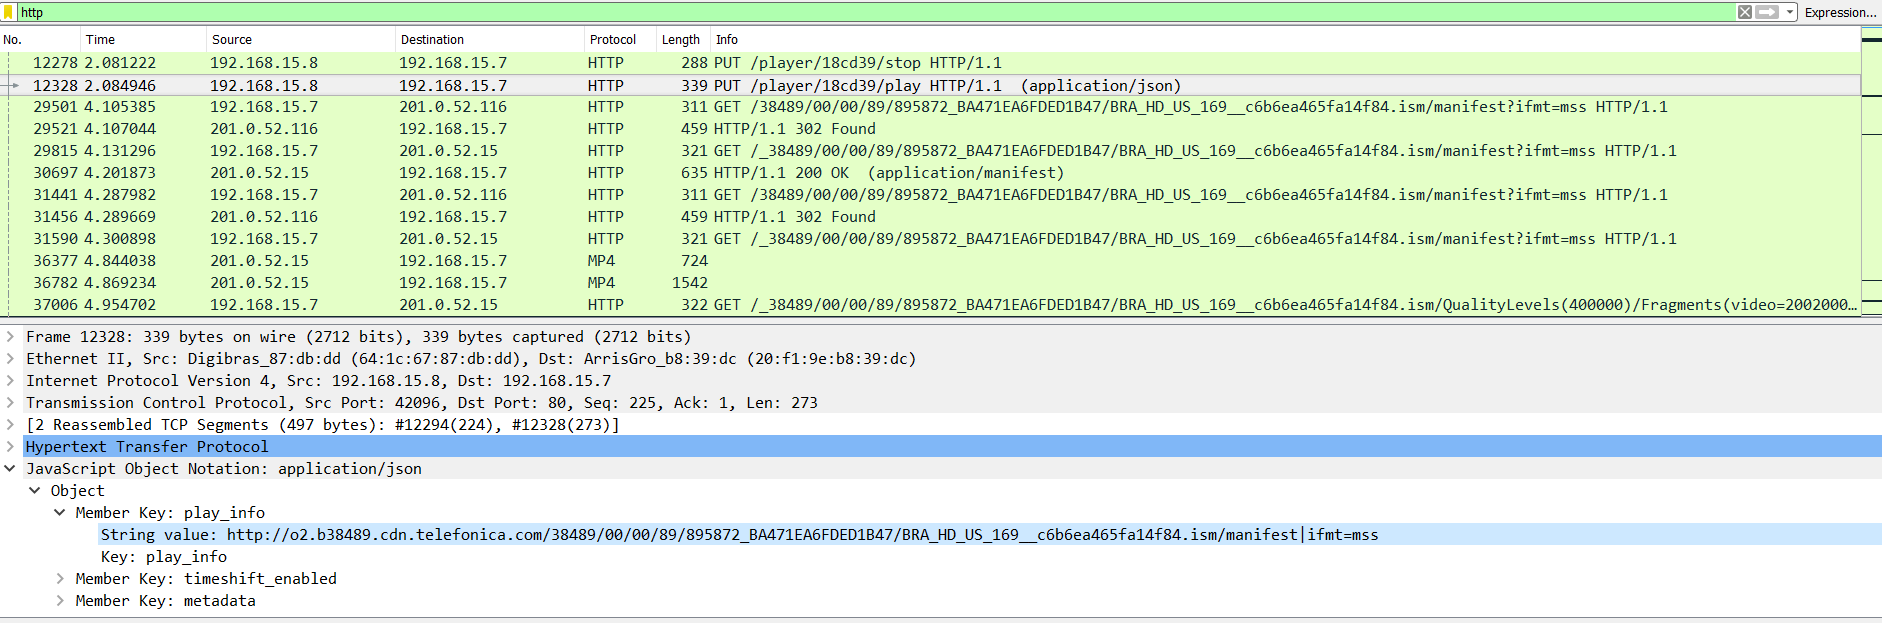
\includegraphics[height=8cm]{Figuras/exemplo_vod_1.png} 
\label{figura:exemplo_vod_1}
\end{figure}

O player, por sua vez, como respons\'avel por enviar as requisi\c{c}\~oes, envia ao servidor principal a requisi\c{c}\~ao do manifest do VOD que ele quer tocar. Figura \ref{figura:exemplo_vod_2}.
\begin{figure}[H]
\caption{exemplo VOD}
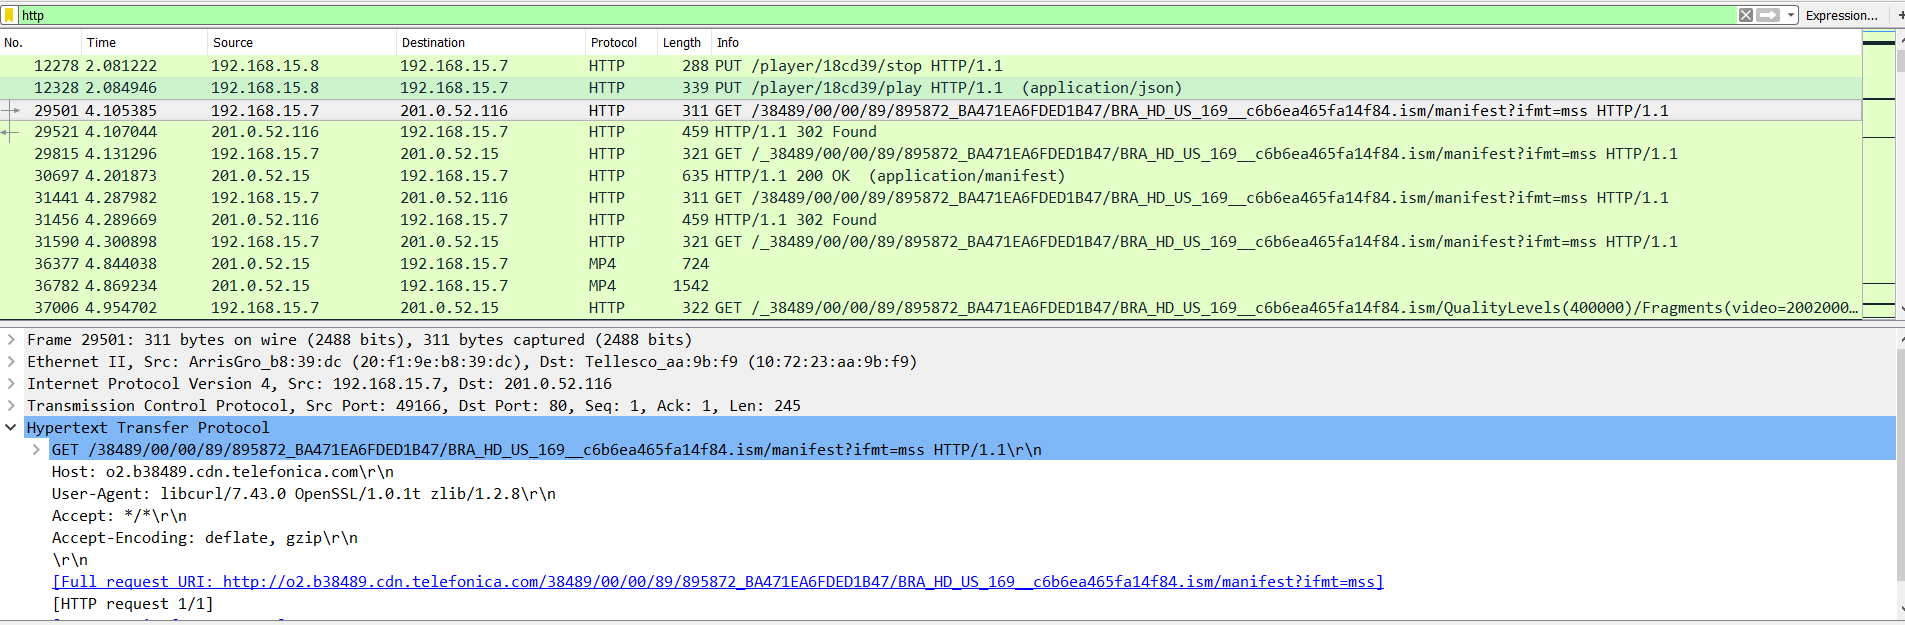
\includegraphics[height=9cm]{Figuras/exemplo_vod_2.png} 
\label{figura:exemplo_vod_2}
\end{figure}

Na figura \ref{figura:exemplo_vod_3} vemos a CDN, que j\'a fez um roteamento para uma outra rede(ou servidor), que retornou com um c\'odigo 302 indicando que o retorno da requisi\c{c}\~ao n\~ao \'e a resposta final. Dentro do cabe\c{c}alho da resposta tem um campo chamado "location" o qual \'e respons\'avel por retornar o endere\c{c}o final (ou intermedi\'ario) para nova requisi\c{c}\~ao. Esse processo ser\'a repetido at\'e o c\'odigo de retorno da requisi\c{c}\~ao for 200.
\begin{figure}[H]
\caption{exemplo VOD}
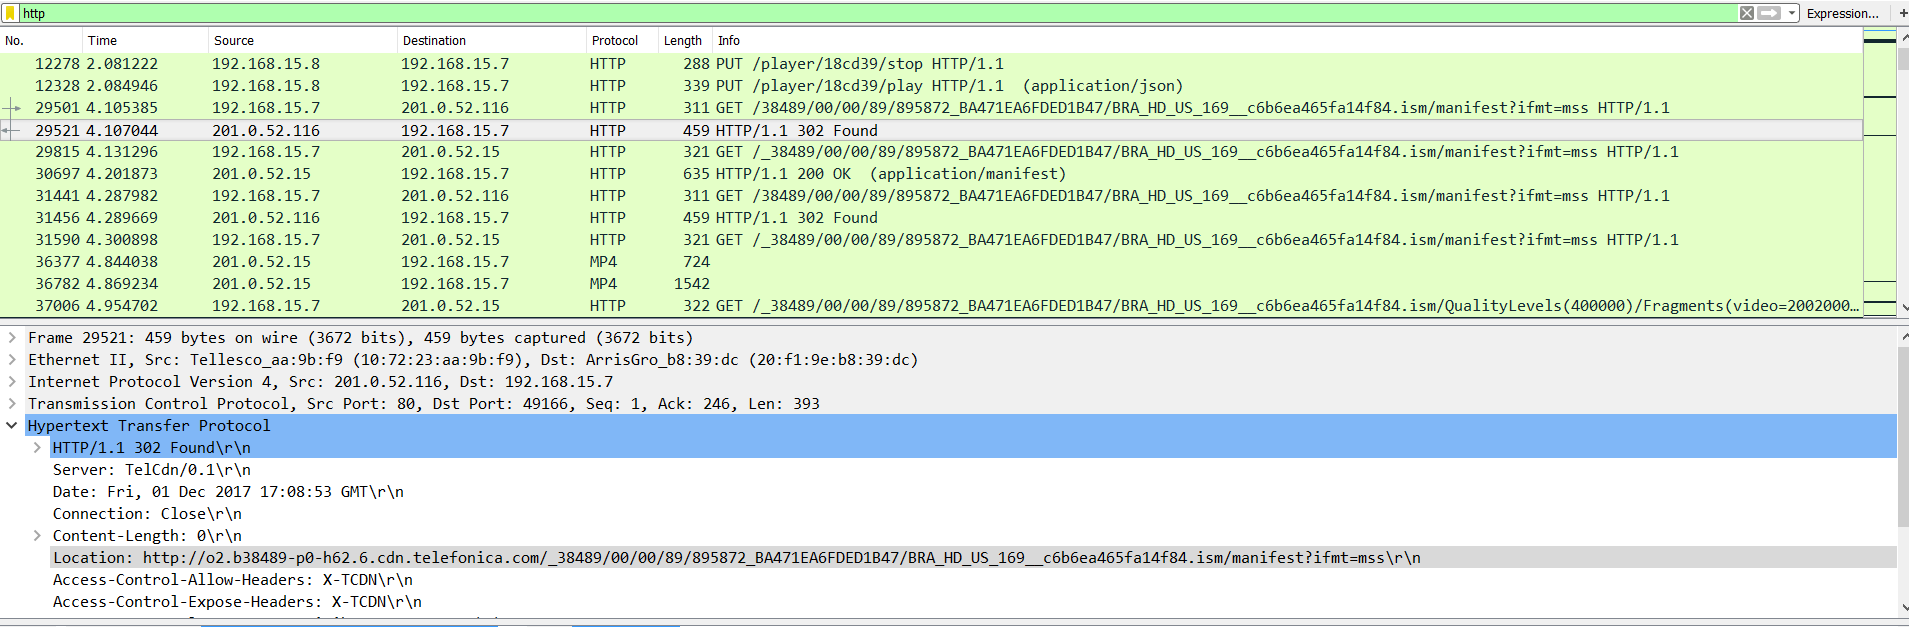
\includegraphics[height=9cm]{Figuras/exemplo_vod_3.png} 
\label{figura:exemplo_vod_3}
\end{figure}

Ainda na figura \ref{figura:exemplo_vod_3} podemos observar que ele recebe um 200 OK da requisi\c{c}\~ao em seguida do 302 Found. O que simboliza que aquela URL \'e a URL final e o player pode utiliza-la como base do manifesto. 

\begin{figure}[H]
\caption{exemplo VOD}
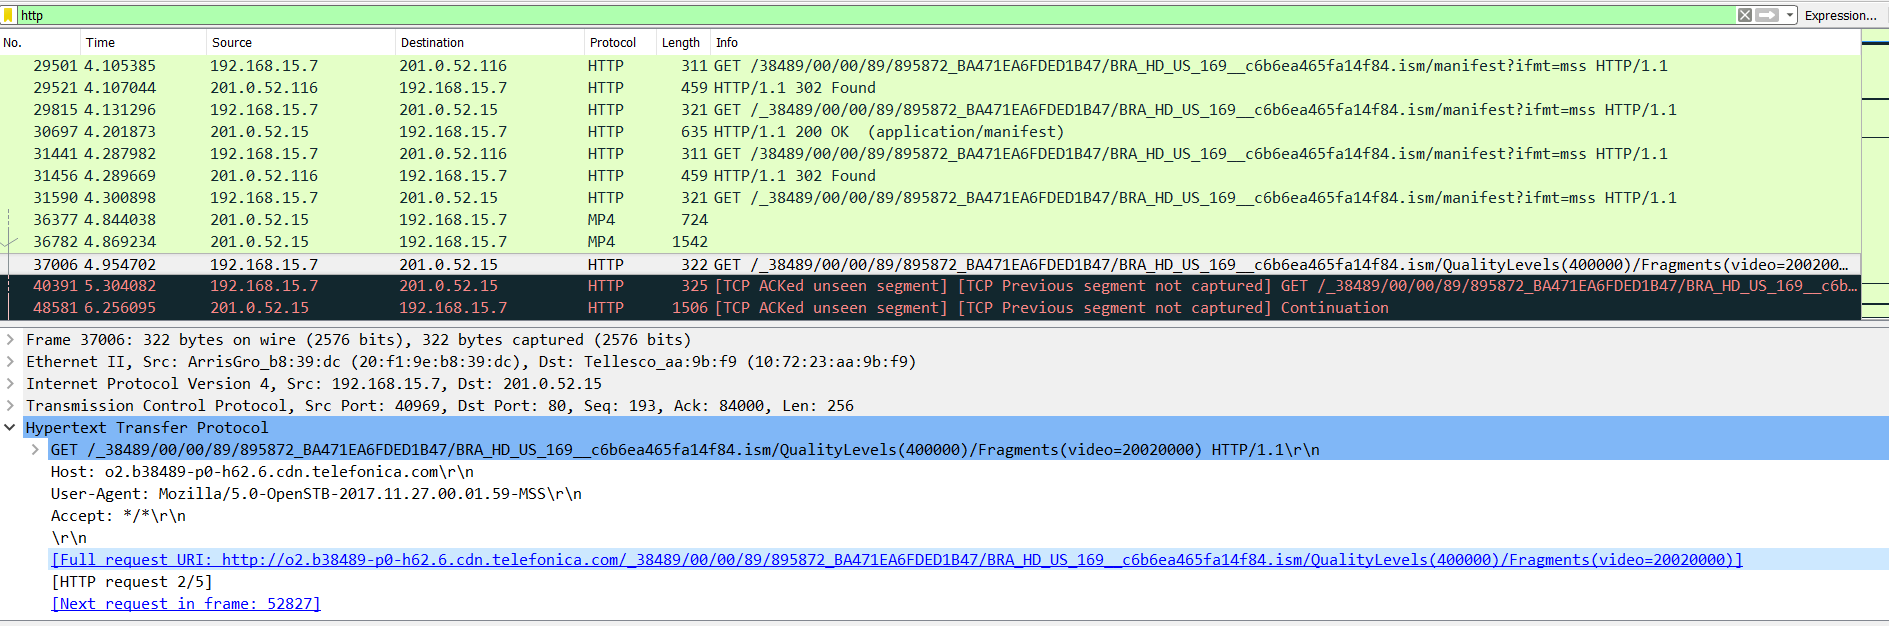
\includegraphics[height=9cm]{Figuras/exemplo_vod_4.png}
\label{figura:exemplo_vod_4}
\end{figure}

Em \ref{figura:exemplo_vod_4} vemos o player come\c{c}ando a consumir os "chuncks" e por consequ\^encia tocando o v\'ideo.